%!TEX root = dippa.tex
%%% This file contains the Gene expression section of my master's thesis.
%%% This section covers the basics of gene expression.
%%% Author: Viljami Aittomäki

\section{Gene expression}\label{gene-expression}

Genetic information is encoded in deoxyribonucleic acid (DNA). A
gene is a section of DNA that serves as a template for a functional
ribonucleic acid (RNA) molecule. Gene expression refers to this process of
synthesizing a functional end-product from the information contained in gene.
DNA and gene expression serve as the basis of all currently known life. \citep{Strachan2011}

Most of gene expression is dedicated to production of proteins. The Central
Dogma of Molecular Biology, postulated by Francis Crick in 1970, describes the
general schema of how genetic information flows from genes to proteins; DNA is
first transcribed into messenger RNA (mRNA), which is then translated into
polypeptides, which ultimately form proteins \citep{Crick1970} (illustrated in
Figure \ref{fig:central-dogma}). The flow is not strictly one-directional,
though, as reverse transcriptases, a family of enzymes, can synthesize DNA
from an RNA template.

\begin{figure}[!h]
  \centering
  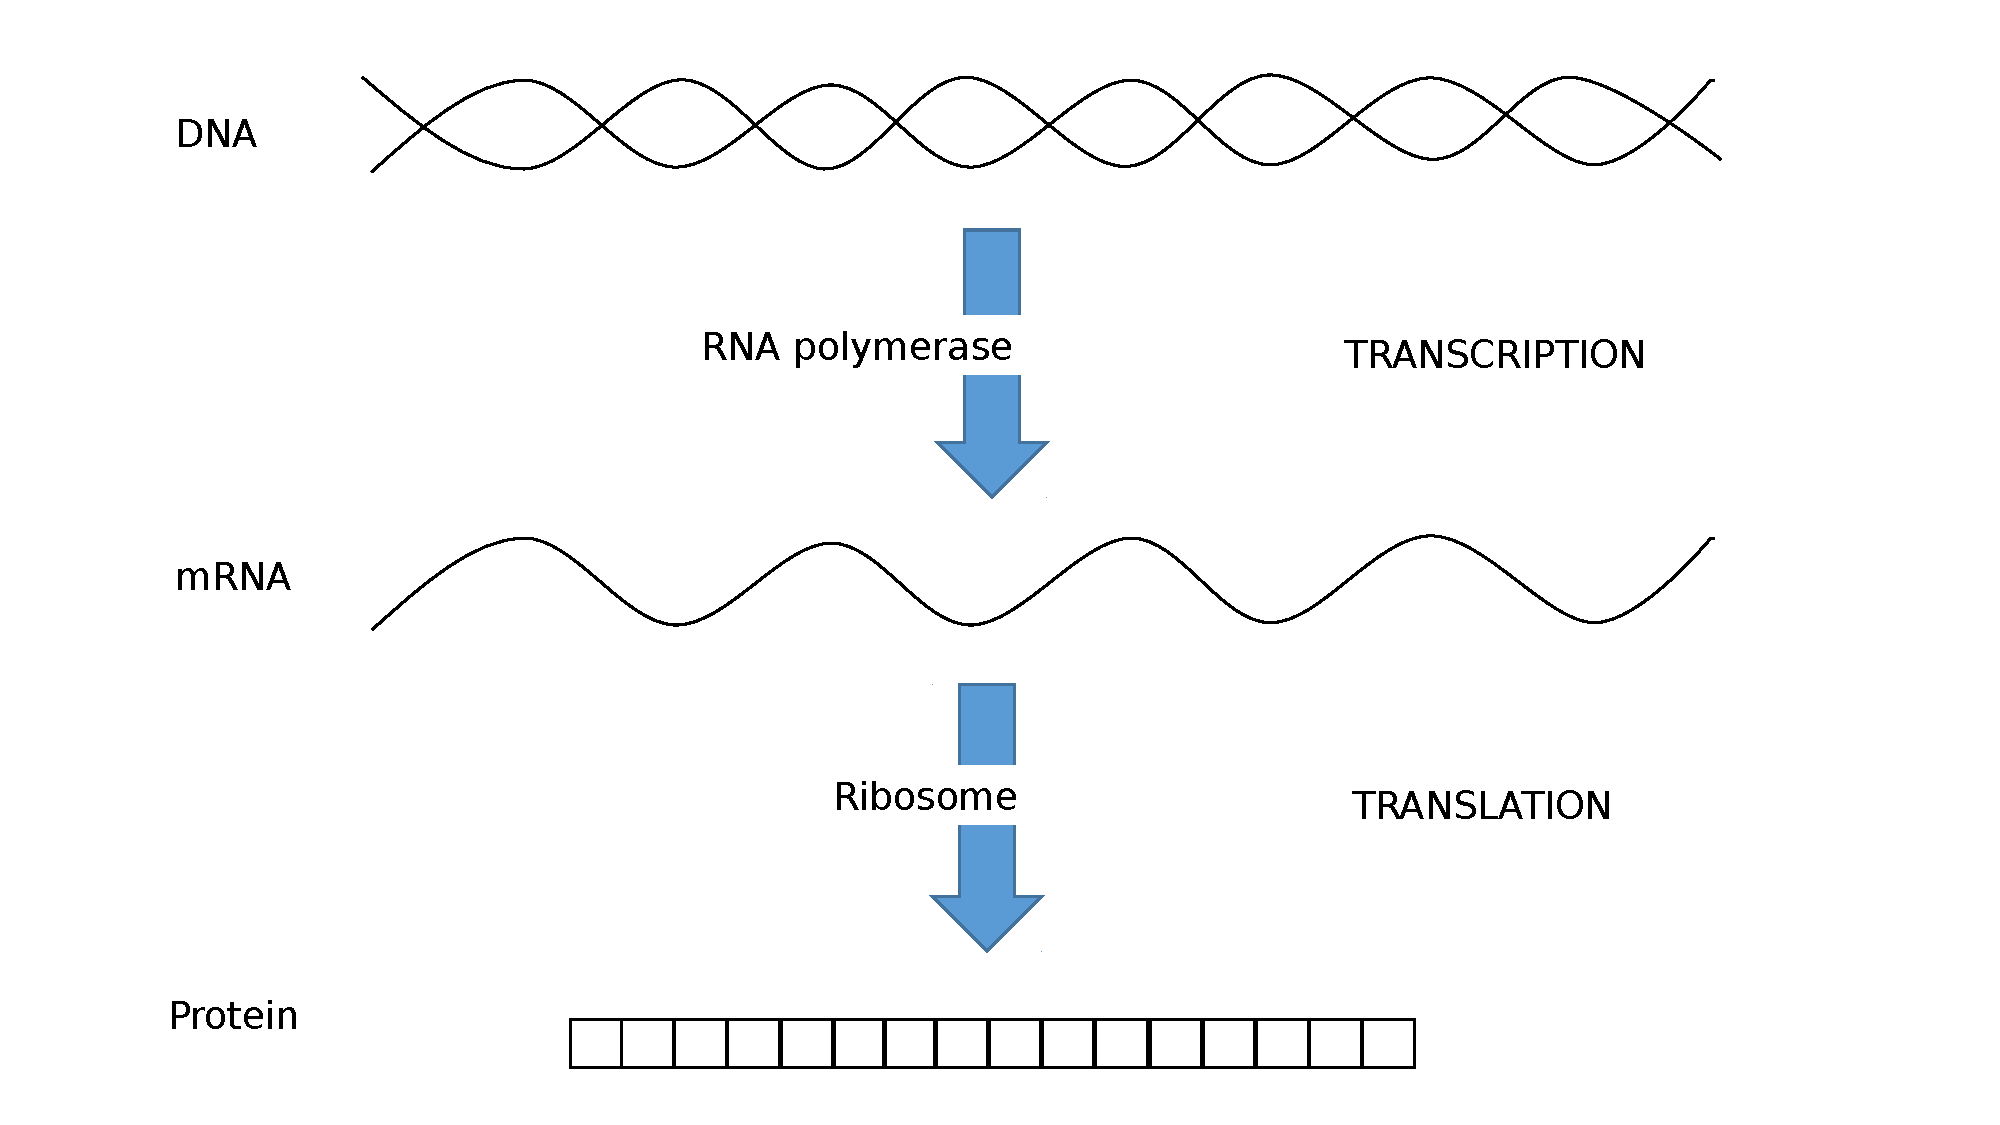
\includegraphics[width=.8\linewidth]{figures/central_dogma.pdf}
  \caption{The Central Dogma of Molecular Biology, as postulated by Crick \citep{Crick1970}.
  Most genetic information flows from DNA to RNA to protein.}
  \label{fig:central-dogma}
\end{figure}

All genes are transcribed to RNA, but all do not encode proteins. The
human genome\footnote{The genome refers to the whole genetic material of an
organism or an individual.} has been suggested to contain approximately 20 500
protein-coding genes, which encompass only around 1.5\% of the whole genetic
sequence \citep{Clamp2007}. The vast majority of the human genome was, thus,
previously thought to be without function and referred to as "junk DNA". More
recently, however, it has become evident that human DNA is pervasively
transcribed, the majority of it appears functional, and many coding and
non-coding regions overlap in the DNA \citep{Strachan2011}.

Non-coding genes give rise to non-coding RNA (ncRNA), a class of RNA molecules
that both participate in and regulate the expression of other genes.
Examples of known ncRNAs and their functions are presented in Table
\ref{table:rnas}. Nevertheless, the function and significance (if any) of many
transcribed and non-coding regions of the genome still remains unknown.

\begin{table}
  \caption{Examples of known major classes of human non-coding RNA and their
  general functions. This table is not exhaustive and several additional classes have
  been discovered. Table adapted from \citep{Strachan2011}. \\
  Size: approximate sequence lengths of each class in number of nucleotides.
  Abbrev.: abbreviations commonly used.}
  \label{table:rnas}
  \centering
  {\fontfamily{lmss}\fontsize{10pt}{12pt}\selectfont
  \begin{tabular}{ lllp{6cm} }
    \hline
    \textbf{RNA class} & \textbf{Abbrev.} & \textbf{Size (nt)} & \textbf{Function} \\
    \hline
    Ribosomal RNA         & rRNA   & 120--5000  & Components of ribosomes (which perform translation) \\
    Transfer RNA          & tRNA   & 70--80     & Transporting peptides and decoding mRNA sequence into peptides \\
    Small nuclear RNA     & snRNA  & 60--360    & Intron splicing; regulation of transcription, chromosomal replication and cell cycle etc.  \\
    MicroRNA              & miRNA  & 21--24     & Post-transcriptional gene regulation \\
    Small interfering RNA & siRNA  & 21--22     & Post-transcriptional regulation \\
    Long non-coding RNA   & lncRNA & $>$ 1000   & Gene regulation at several stages \\
    \hline
  \end{tabular}
  }
\end{table}




\subsection{Regulation of gene expression}\label{regulation-of-gene-expression}

The proper regulation of gene expression is paramount for cells
to respond to external signals, changes in their environment, and 
go through different developmental stages. Gene expression can be regulated
at any stage of the process, and regulation can be roughly divided into transcriptional
and post-transcriptional regulation.

Transcriptional regulation with e.g. TFs, methylation, adenylation, splicing.

Post-transcriptional

MicroRNAs (miRNAs) and small interfering RNAs (siRNAs) are components of the
so called RNA interference (RNAi) pathway, which is a mechanism for regulating
gene expression post-transcriptionally. miRNAs and siRNAs are practically
interchangeable as substrates for RNAi, both act as target mRNA recognizing
templates, but have different biogenesis. While miRNAs are cut from endogenous
hairpin structures and siRNAs are mostly processed from exogenous long double-
stranded RNAs (dsRNAs). \cite{Du2005} MicroRNAs, which are the focus of this study,
are discussed in more detail in the next section.

% The Argonaute (Ago) family of proteins is closely associated with small RNAs and
% Ago act as effectors in RNAi \cite{Ha2014}.

\begin{itemize}
  \item transcription factors
  \item post-transcriptional regulation
  \item translational factors
  \item protein degradation
\end{itemize}




\subsection{Measuring gene expression}\label{measurement-of-gene-expression}

The physical measurement of gene expression can be done on either the level of
messenger RNA molecules or protein molecules. Although proteins are the
eventual effectors molecules within cells -- at least for protein-coding genes
-- gene expression is usually thought to be synonymous with mRNA expression.
mRNA abundances are significantly easier than
measuring protein abundances, due to the chemistry of base-pair formation and
the relative ease of replicating DNA (or RNA) sequences by exploiting cellular
machinery evolved for this purpose.

Techniques shortly in one paragraph:
\begin{itemize}
  \item blotting, qPCR
  \item microarrays
  \item sequencing-based methods
  \item protein arrays (RPPA)
\end{itemize}




\subsubsection{Microarrays}

\begin{itemize}
  \item basics of operation
  \item shortly on microarray analysis
  \begin{itemize}
    \item preprocessing and normalization
    \item probe annotation problems
  \end{itemize}
\end{itemize}

The general assumption has been that mRNA expression is representative of gene
expression and that changes in mRNA abundances also reflect changes in protein
abundances and. This assumption has recently been challenged by experiments
indicating that correlation between the expression of mRNA and corresponding
protein low, with mRNA expression explaining around 40\% of variation in
protein abundances \citep{Vogel2012}. There are also contrary findings of
modest to good correlation and one study suggested that mRNA-protein
correlations are generally higher for genes that have differing mRNA
expression between studied conditions (e.g. cancerous versus healthy tissue)
\citep{Koussounadis2015}, suggesting that, while correlation is perhaps low in
general, changes in mRNA expression cause detectable changes in protein
expression.

Nonetheless, Payne recently concluded that "proteome and transcriptome
abundances are not sufficiently correlated to act as proxies for each other"
and that most of this difference is likely caused by biological regulation and
not by measurement technology \cite{Payne2015}.
% This regulation can be post-transcriptional, translational
% or protein-degradation related, as discussed above.
Therefore, it is interesting, even necessary, to integrate measurements from
different stages of gene expression -- for example mRNA, microRNA and protein
abundances -- to gain new insights into biological processes.
